%&preamble

\newcommand{\versuch}{Operational Amplifiers}
\newcommand{\versuchsnr}{59}			%P!- weglassen
\newcommand{\fehlerrechnung}{Nein}

\newcommand{\betreuer}{Johann Frank}
\newcommand{\durchgefuehrt}{08.06.17}

\newcommand*\comp[1]{\ensuremath{\mathrm{#1}}}	%used for components, eg \comp{R_1}
\newcommand*\ua{\ensuremath{U_\text{A}}}
\newcommand*\ue{\ensuremath{U_\text{E}}}
\newcommand*\diff{\mathop{}\!\mathrm{d}}
\newcommand{\at}[2][]{#1|_{#2}}

\begin{document}
	\FrontMatter
	% coordinates for background border
\newcommand{\diameter}{20}
\newcommand{\xone}{-15}
\newcommand{\xtwo}{160}
\newcommand{\yone}{15}
\newcommand{\ytwo}{-253}

\newcommand{\hoehea}{60}
\newcommand{\hoeheb}{60}




\begin{titlepage}
    % background border
    \begin{tikzpicture}[overlay]
    \draw[color=gray]  
            (\xone mm, \yone mm)
      -- (\xtwo mm, \yone mm)
    arc (90:0:\diameter pt) 
      -- (\xtwo mm + \diameter pt , \ytwo mm) 
        -- (\xone mm + \diameter pt , \ytwo mm)
    arc (270:180:\diameter pt)
        -- (\xone mm, \yone mm);
    \end{tikzpicture}
    
    % KIT logo
    \begin{textblock}{10}[0,0](4.5,2.5)
        
\includegraphics[width=.25\textwidth]{../praktikum-protokollvorlage-latex/include/kitlogo.pdf}
    \end{textblock}
    \changefont{phv}{m}{n}    % helvetica
    \begin{textblock}{10}[0,0](5.5,2.2)
        \begin{flushright}
            \Large FAKULTÄT FÜR PHYSIK\\Praktikum Klassische Physik
        \end{flushright}
    \end{textblock}
    
    \begin{textblock}{10}[0,0](4.2,3.1)
        \begin{tikzpicture}[overlay]
        \draw[color=gray]
            (\xone mm + 5 mm, -12 mm)
         -- (\xtwo mm + \diameter pt - 5 mm, -12 mm);
        \end{tikzpicture}
    \end{textblock}
    
    \Large
    % Zeile 1
    \begin{textblock}{12}[0,0](3.58,4.4)
        \mytextfield{Prak.}{\praktikum}{0.9cm}{17pt}
                    {P1/P2}{2}{Praktikum}
    \end{textblock}
    \begin{textblock}{12}[0,0](5.53,4.4)
        \mytextfield{Semester}{\semester}{2.6cm}{17pt}
        {z.B. \glqq WS14/15\grqq\ oder \glqq SS15\grqq}{0}{Semester}
    \end{textblock}
    \begin{textblock}{12}[0,0](9.53,4.4)
        \mytextfield{Wochentag}{\wochentag}{1.3cm}{17pt}
                    {Mo/Di/Mi/Do}{2}{Wochentag}
    \end{textblock}
    \begin{textblock}{12}[0,0](12.88,4.4)
       \mytextfield{Gruppennr.}{\gruppennr}{1.06cm}{17pt}
                   {\#\#}{2}{Gruppennummer}
    \end{textblock}
    
    % Zeile 2
    \begin{textblock}{12}[0,0](3.58,4.95)
        \mytextfield{Name}{\nachnamea}{6cm}{17pt}
                    {}{0}{Name1}
    \end{textblock}
    \begin{textblock}{12}[0,0](9.53,4.95)
        \mytextfield{Vorname}{\vornamea}{6cm}{17pt}
                    {}{0}{Vorname1}
    \end{textblock}
    
    % Zeile 3
    \begin{textblock}{12}[0,0](3.58,5.5)
        \mytextfield{Name}{\nachnameb}{6cm}{17pt}
                    {}{0}{Name2}
    \end{textblock}
    \begin{textblock}{12}[0,0](9.53,5.5)
        \mytextfield{Vorname}{\vornameb}{6cm}{17pt}
                    {}{0}{Vorname2}
    \end{textblock}
    
    % Zeile 4
    \begin{textblock}{12}[0,0](3.64,6.05)
       \normalsize\mytextfield{Emailadresse(n)}{\emailadressen}{13.1cm}{10pt}
                              {Optional}{0}{Emailadressen}
    \end{textblock}
    
    % Zeile 5
    \begin{textblock}{12}[0,0](3.58,7)
        \mytextfield{Versuch}{\versuch\ (\praktikum-\versuchsnr)}{9.45cm}{14pt}
                    {z.B. \glqq Galvanometer (P1-13)\grqq\ oder \glqq %
                     Mikrowellenoptik (P2-15)\grqq}{0}{Versuch}
    \end{textblock}
    \begin{textblock}{12}[0,0](12.58,7)
       \mytextfield{Fehlerrech.}{\fehlerrechnung}{1.46cm}{17pt}
                   {Ja/Nein}{4}{Fehlerrechnung}
    \end{textblock}
    
    % Zeile 6
    \begin{textblock}{12}[0,0](3.58,7.55)
        \mytextfield{Betreuer}{\betreuer}{7cm}{17pt}{}{0}{Betreuer}
    \end{textblock}
    \begin{textblock}{12}[0,0](10.82,7.55)
        \mytextfield{Durchgeführt am}{\durchgefuehrt}{2.53cm}{17pt}
                    {TT.MM.JJ}{8}{Durchfuehrung}
    \end{textblock}
    
    % Querstrich
    \begin{textblock}{20}[0,0](0,7.9)\tiny\centering
        Wird vom Betreuer ausgefüllt.
    \end{textblock}
    \begin{tikzpicture}[overlay]
    \draw[color=gray]
        (\xone mm + 5 mm, -95 mm)
     -- (\xtwo mm + \diameter pt - 5 mm, -95 mm);
    \end{tikzpicture}
    
    % Zeile 1
    \begin{textblock}{12}[0,0](3.65,8.57)
        \myTtextfield{1. Abgabe am}{}{2.5cm}{17pt}
                     {}
    \end{textblock}
    
    % Block 1
    \begin{tikzpicture}[overlay]
    \draw[color=gray]  
        (\xone mm + 10 mm, -107.5 mm)
     -- (\xtwo mm + \diameter pt - 10 mm, -107.5 mm)
     -- (\xtwo mm + \diameter pt - 10 mm, -107.5 mm - \hoehea mm)
     -- (\xone mm + 10 mm, -107.5 mm - \hoehea mm)
     -- (\xone mm + 10 mm, -107.5 mm);
    \end{tikzpicture}
    \begin{textblock}{20}[0,0](3.8,9.2)
        \myTtextfield{Rückgabe am}{}{2.5cm}{17pt}
                     {}
    \end{textblock}
    \begin{textblock}{20}[0,0](8.7,9.2)
        \smash{Begründung:}
    \end{textblock}
    
    % Zeile 2
    \begin{textblock}{12}[0,0](3.65,12.6)
        \myTtextfield{2. Abgabe am}{}{2.5cm}{17pt}
                     {}
    \end{textblock}
    
    % Block 2
    \begin{tikzpicture}[overlay]
    \draw[color=gray]  
        (\xone mm + 10 mm, -180 mm)
     -- (\xtwo mm + \diameter pt - 10 mm, -180 mm)
     -- (\xtwo mm + \diameter pt - 10 mm, -180 mm - \hoehea mm)
     -- (\xone mm + 10 mm, -180 mm - \hoehea mm)
     -- (\xone mm + 10 mm, -180 mm);
    \end{tikzpicture}
    \begin{textblock}{12}[0,0](4,13.25)
        \smash{Ergebnis:~~~~+~~~/~~~0~~~/~~~-}
    \end{textblock}
    \begin{textblock}{12}[0,0](9.5,13.25)
        \smash{Fehlerrechnung:~~~Ja~~~/~~~Nein}
    \end{textblock}
    \begin{textblock}{12}[0,0](3.8,13.72)
        \myTtextfield{Datum}{}{2.5cm}{17pt}
                     {}
    \end{textblock}
    \begin{textblock}{12}[0,0](8.3,13.72)
        \myTtextfield{Handzeichen}{}{5.5cm}{17pt}
                     {}
    \end{textblock}
    \begin{textblock}{12}[0,0](4,14.25)\Large
        \smash{Bemerkungen:}
    \end{textblock}
    
    
    
    % lowest text blocks concerning the KIT
    \begin{textblock}{10}[0,0](4,16.8)
        \tiny{KIT -- Universität des Landes Baden-Württemberg und nationales %
              Forschungszentrum in der Helmholtz-Gemeinschaft}
    \end{textblock}
    \begin{textblock}{10}[0,0](14,16.75)
        \large{\textbf{www.kit.edu}}
    \end{textblock}
\end{titlepage}

	\maketitlepage

	\MainMatter

	\chapter{Theory}

	\chapter{Common emitter amplifier}
This experiment explores the usage of a transistor as an amplifier.

\section{Theory}\label{sec:theory}
\begin{figure}[tbp]
	\centering
	%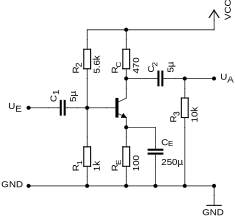
\includegraphics[width=.5\textwidth]{./img/com_emitter_amp.pdf}
	\caption[Single Stage Common Emitter Amplifier]{Single stage common emitter amplifier}
	\label{fig:com_emitter_amp}
\end{figure}
The circuit shown in \autoref{fig:com_emitter_amp} acts as an inverting voltage amplifier.
The input and output capacitors remove any DC component of the input.
\comp{R_1} and \comp{R_2} are used to bias the transistor, so that it remains in active mode during operation.
This method of biasing vastly reduces the effects of varying $\beta$ as a cause of temperature drift by holding the base bias at a constant voltage.
Adversely, the constant voltage at the base introduces a stronger dependency on the base-emitter voltage drop, which changes by \SI{-2}{\milli\volt\per\kelvin}.
\comp{R_E} is used to compensate for this by introducing negative feedback, albeit lowering the gain.

Temperature drift can be calculated as
\begin{equation}
	\frac{\d U_\text{a}}{\d T}=\frac{\d U_\text{a}}{\d U_\text{e}}\frac{\d U_\text{e}}{\d T}\approx A\cdot\SI{-2}{\milli\volt\per\kelvin},
\end{equation}

where $U_\text{a}$ denotes the output voltage, $U_\text{e}$ the input voltage and $T$ the temperature.
This means that temperature drift is proportional to the gain $A$ in a common emitter amplifier.
As temperature drift happens slowly, only DC amplification has to be decreased, whereas AC amplification can remain unchanged.
This can be realized by putting a capacitor \comp{C_E} in parallel to the emitter resistor \comp{R_E} which will decrease the negative feedback with growing frequency.

The quiescent base voltage is determined by the voltage divider formed by \comp{R_1} and \comp{R_2}:
\begin{equation}\label{eq:bias_volt}
	V_\text{bias}=V_\text{cc}\cdot\frac{\comp{R_2}}{\comp{R_1}+\comp{R_2}}.
\end{equation}

\begin{figure}[tbp]
	\centering
	%\includegraphics[width=.5\textwidth]{./img/small_signal_neg_feed.pdf}
	\caption{Small signal schematic of a common emitter circuit with negative feedback}
	\label{fig:small_signal_neg_feed}
\end{figure}

To deduce a proper formula for the AC-voltage amplification of a common emitter circuit with negative feedback, let us consider the small signal equivalent schematic seen in \autoref{fig:small_signal_neg_feed}.
The transistor can be replaced by a constant current source with differential resistances \comp{r_{BE}} and \comp{r_{CE}}.
Using \texttt{Kirchhoff}'s law for nodes, it holds
\begin{alignat}{2}
	\frac{u_\text{e}-u_\text{E}}{r_\text{BE}}+Su_\text{BE}+\frac{u_\text{a}-u_\text{E}}{r_\text{CE}} &= \frac{u_\text{E}}{R_\text{E}} \label{eq:small_1}\\
	Su_\text{BE}+\frac{u_\text{a}-u_\text{E}}{r_\text{CE}} + \frac{u_\text{a}}{R_\text{C}}&= i_\text{a}, \label{eq:small_2}
\end{alignat}
where $S=\frac{I_\text{C}}{U_\text{T}}$ denotes the transistor's conductance.
Rearraging equations \ref{eq:small_1}, \ref{eq:small_2} and using $u_\text{BE}=u_\text{e}-u_\text{E}$, this yields
\begin{align}
	A&=\frac{u_\text{a}}{u_\text{e}}\at[\bigg]{i_\text{a}=1} \nonumber \\
	&=-\frac{SR_\text{C}\left(1-\frac{R_\text{E}}{\beta r_\text{CE}}\right)}{1+R_\text{E}\left(S\cdot\left(1+\beta^{-1}+\frac{R_\text{C}}{\beta r_\text{CE}}\right)+r_\text{CE}^{-1}\right)+\frac{R_\text{C}}{r_\text{CE}}} \nonumber \\
	&\approx -\frac{SR_\text{C}}{1+SR_\text{E}}, \label{eq:amp_neg_fb}
\end{align}
where $r_\text{CE}\gg R_\text{C},R_\text{E}$, $\beta\gg 1$, $S$ denotes conductance of the transistor and $\beta$ its current amplification $\frac{I_\text{c}}{I_\text{B}}$.
\section{Evaluation}
\begin{figure}[tbp]
	\centering
	%\includegraphics[width=.5\textwidth]{./img/com_emitter_in_out.pdf}
	\caption{Input versus output voltage}
	\label{fig:com_emitter_in_out}
\end{figure}
\begin{table}[b!]
	\centering
	\caption{Input, output voltages $V_\text{pp,in/out}$ and resulting voltage amplification $A$ at $f=\SI{1}{\kilo\hertz}$}
	\label{tab:com_emit_in_out}
	\begin{tabular}{S|SSS}
		\toprule
		{}&	{$V_\text{pp,in}$ in $\si{\milli\volt}$}&	{$V_\text{pp,out}$ in $\si{\volt}$}&	{$A$}\\
		\midrule
		{with \comp{C_e}}	&	\num{19}	&	\num{2.7}	&	\num{-142}\\
		{}	&	\num{68}	&	\num{10.3}	&	\num{-151}\\
		\midrule
		{without \comp{C_e}}	&	\num{70.8}	&	\num{0.322}	&	\num{-4.55}\\
		{}	&	\num{278}	&	\num{1.3}	&	\num{-4.676}\\
		\bottomrule
	\end{tabular}
\end{table}
The circuit \autoref{fig:com_emitter_amp} is built (including the emitter capacitor, which is taken out later on) and a triangular input signal is applied.
\autoref{fig:com_emitter_in_out} shows the measured voltage curves for input and output voltage.
Minimal non-linearities in the amplified output signal can be observed.
\autoref{tab:com_emit_in_out} lists measured peak-to-peak voltages and resulting voltage amplifications.
Using \autoref{eq:bias_volt} the bias voltage can be calculated as $U_\text{bias}=\SI{2.27}{\volt}$.
Assuming that the base current is negligable, the collector current is $I_\text{c}\approx\frac{U_\text{bias}-\SI{0.7}{\volt}}{\comp{R_E}}=\SI{15.7}{\milli\ampere}$.
Using $I_\text{c}$, we can calculate the conductance to be $S=\frac{I_\text{c}}{U_\text{T}}=\SI{604}{\milli\siemens}$.
The condcutance can then be utilized to finally calculate the theoretical voltage amplification \textbf{without capacitor $\comp{C_E}$} by using the formula derived in \autoref{eq:amp_neg_fb}.
\begin{align*}
	A &= -\frac{SR_\text{C}}{1+R_E} \\
	&=\num{-4.63}.
\end{align*}
With \comp{C_E}, however, the amplification is expected to rise further up to $A=-S\cdot R_\text{C}=\num{283.88}$, which corresponds to the AC-amplification value of a common emitter circuit without negative feedback.
The cutoff frequency of the high-pass formed by \comp{R_E} and \comp{C_E} can be calculated by
\begin{align*}
	f_\text{cutoff}&=\frac{1}{2\pi R_\text{E}C_\text{E}}	\\
	&=\SI{6.37}{\hertz}.
\end{align*}
This means that for frequencies vastly over $f_\text{cutoff}$ negative feedback does not apply anymore.
\begin{figure}[tbp]
	\centering
	\includegraphics[width=.7\textwidth]{./data/plots/1_4.pdf}
	\caption{Amplification $A$ over Frequency $f$}
	\label{fig:com_emitter_freq}
\end{figure}
\begin{table}[b!]
	\centering
	\caption{Input, output voltages $U_\text{in/out}$ at different frequencies $f$}
	\label{tab:com_emit_freq}
	\begin{tabular}{S|SS|SS}
		\toprule
		{Frequency in $\si{\kilo\hertz}$}&
		{$U_\text{in}$ in $\si{\milli\volt}_\text{pp}$}&
		{$U_\text{out}$ in $\si{\volt}_\text{pp}$}&
		{$U_\text{in,cap}$ in $\si{\milli\volt}_\text{pp}$}&
		{$U_\text{out,cap}$ in $\si{\volt}_\text{pp}$}\\
		\midrule
		0.01    &  368  &   0.316  & 40   &   0.4	\\
		0.025   &   416   &  0.688 &  50   &   1	\\
		0.05   &   416   &  1.2   &  51   &  1.66	\\
		0.1  &   416   &  1.7   &  51   &   2.6	\\
		0.5  &   416   &  2     &  50   &   7	\\
		1  &   416   &  2     &  47   &   8	\\
		5  &   416   &  2     &  47   &   8.5	\\
		10 &   408  & 1.96  &  48   &   8.6	\\
		50 &   432  &   2.10  &  47   &   8.3	\\
		100  & 432   &  2.12  &  47   &   8	\\
		\bottomrule
	\end{tabular}
\end{table}

To examine this statement, a sinusoidal signal of varying frequency is applied and input and output voltages are measured to determine the voltage amplification $A$.
\autoref{fig:com_emitter_freq} shows the amplifcation calculated from \autoref{tab:com_emit_freq} over frequency $f$.
As expected, without \comp{C_E} the amplification remains almost constant.

With \comp{C_E}, however, the amplification gradually increases until it reaches its maximum at $\approx\num{176}$, which deviates from the theoretical value of \num{283.88}.
This result may be explained by the ESR (\textbf{E}quivalent \textbf{S}eries \textbf{R}esistance) of \comp{C_E} which poses a residual resistance at high frequencies instead of the capacitor being a short circuit.
Furthermore, the conductance of the transistor in a common emitter circuit without negative feedback differs from the conductance in the examined circuit in that the base current changes with \comp{R_E} not being present.

The highpass frequency response function
\begin{equation*}
	A=\frac{A_0}{\sqrt{1 + (2\pi f\tau)^{-2}}}
\end{equation*}
is fitted to the data with \comp{C_E}, as explained in \autoref{sec:theory}.
A fit parameter of $\tau=\SI{481.3e-6}{\second}^{-1}$ is determined, which deviates from the theoretical value of $RC=\SI{25e-3}{\second}^{-1}$ by \SI{98.1}{\percent}.
The exact frequency response is influenced by many factors, such as time constants formed by the AC-coupling capacitors.
See \url{http://whites.sdsmt.edu/classes/ee320/notes/320Lecture23.pdf} (p.13).

	\chapter{Inverting Configurations}
\section{Inverting Amplifier}

\begin{figure}
	\centering
	\begin{subfigure}{0.4\textwidth}
		\centering
		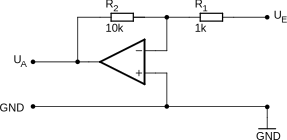
\includegraphics[width=.9\linewidth]{./img/schem-inv.pdf}
		\caption{Basic Inverting Amplifier with Gain 10}
		\label{schem:inv}
	\end{subfigure}
	\begin{subfigure}{0.4\textwidth}
		\centering
		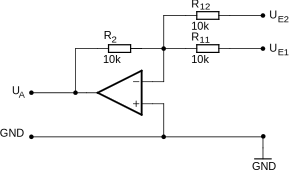
\includegraphics[width=.9\linewidth]{./img/schem-add.pdf}
		\caption{Inverting Adder}
		\label{schem:add}
	\end{subfigure}
\end{figure}

In the inverting configuration shown in \autoref{schem:inv}, the input signal is fed into the feedback loop, the non-inverting input is held at a fixed voltage.
As the opamp is configured for negative feedback, both inputs are held at the same potential which is often ground.
As the inverting input is not directly connected to a voltage source, it's node is called a 'virtual ground'.

Unlike the non-inverting amplifier, the input of the inverting amplifier has a low input impedance, set by \comp{R_1}.

The gain of the circuit is calculated from the current through \comp{R_1} to the virtual ground node: $I_\comp{R_1} = \frac{\ue}{R_1}$, which is equal to the current through \comp{R_2}: $I_\comp{R_2} = \frac{\ua}{R_2}$.
Using a consistent reference direction, the gain  $A$ is \[A = \frac{\ua}{\ue} = -\frac{R_2}{R_1}\].

\section{Inverting Adder}

Ignoring \comp{R_1} in \autoref{schem:inv}, the output voltage \ua is $\ua = -R_2 \cdot I_\text{in}$, with the total current $I_\text{in}$ flowing into the virtual ground node of the inverting input.
As the voltage at this node is independent of $I_\text{in}$, more inputs can be connected, each via a resistor that controls the gain of the respective input.
The individual input currents add up to $I_\text{in}$ and the output voltage is \[\ua = -R_2 \cdot \left(\frac{{\ue}_1}{R_{11}} + \frac{{\ue}_2}{R_{12}} + \dots\right)\] with the component labels shown in \autoref{schem:add}.

	\chapter{Complex Circuits with OpAmps}
\section{Ideal Half-Wave Rectifier}

\begin{figure}
	\centering
	\begin{subfigure}{0.44\textwidth}
		\centering
		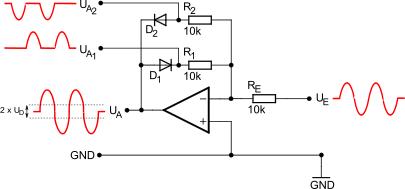
\includegraphics[width=\linewidth]{./img/schem-rectifier.pdf}
		\caption{Ideal Rectifier}
		\label{schem:rectifier}
	\end{subfigure}
	\begin{subfigure}{0.55\textwidth}
		\centering
		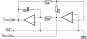
\includegraphics[width=\linewidth]{./img/schem-wavegen.pdf}
		\caption{Square and Triangle Wave Generator}
		\label{schem:wavegen}
	\end{subfigure}
	\caption{}
\end{figure}

A basic half-wave rectifier consists of a diode a resistor to provide a load to the diode.
All diodes carry an inherent voltage drop, so the signal level is lowered by \SI{0.2}{\volt} (Schottky diode) to \SI{0.7}{\volt} (silicon diode).
To combat this amplitude loss, an ideal rectifier is used.

An ideal rectifier (\autoref{schem:rectifier}) uses an operational amplifier with separate feedback paths for the positive and negative half wave.
Looking just at the output of the opamp, the two diodes in the feedback path are essentially anti-parallel, the rest forming an inverting ampifier with gain 1.
As the voltage drop due to the diodes in the feedback path is compensated by the feedback loop, the output of the opamp follows the input, with the amplitude increased by one diode drop.
This means that at zero crossings, in theory the output voltage is discontinuous, introducing high frequency components that may lead to undesired effects.

To now recover the rectified (or more specifically separated) positive and negative half waves, the circuit is tapped in the middle of each feedback line, where the output signal amplitude matches the input signal amplitude (this can be verified by looking at the two identical resistors connected to the inverting input: carrying the same current, they have an equal voltage across them with the inverting input being a virtual ground).

\section{Square and Triangle Wave Generator}

Operational amplifiers can also be operated with positive feedback.
As any perpetuation is amplified and fed back to the input in phase, the output voltage will not remain stable between the rails and is limited only by the rail voltage of the opamp.

By adding the output signal to the input signal, a bistable flip flop with different threshold voltages $U_{\text{thr, H} \rightarrow \text{L}} < U_{\text{thr, L} \rightarrow \text{H}}$, set by \comp{R_1} and \comp{R_2}, is created.
This circuit is called a non-inverting Schmitt trigger, and makes up the right portion of the circuit shown in \autoref{schem:wavegen}.

The left part of the circuit is an inverting integrator, it's output connected to the input of the Schmitt trigger.
As it receives either the positive or negative rail voltage, it acts as a ramp generator and ramps between the two threshold points of the Schmitt-trigger.
The resulting triangle wave is one output signal.
The other output signal is the square wave output of the Schmitt trigger, with a phase of \SI{90}{\degree} relative to the triangle signal.
The output signals are shown in \autoref{ss:wavegen}.

\begin{figure}
	\centering
	\begin{subfigure}{0.4\textwidth}
		\centering
		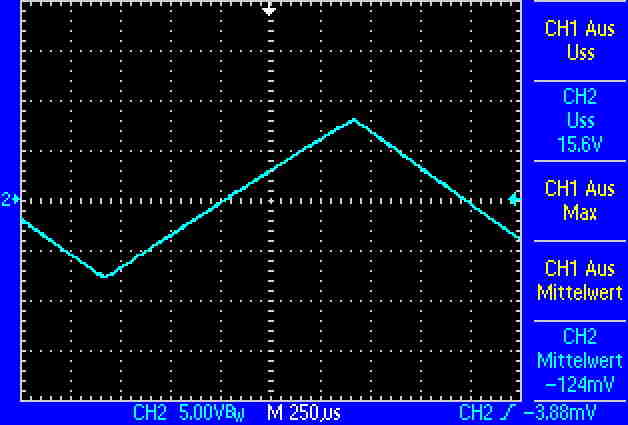
\includegraphics[width=.9\linewidth]{./img/ss-wavegen-triag}
		\caption{Triangle Wave Output Signal}
	\end{subfigure}
	\begin{subfigure}{0.4\textwidth}
		\centering
		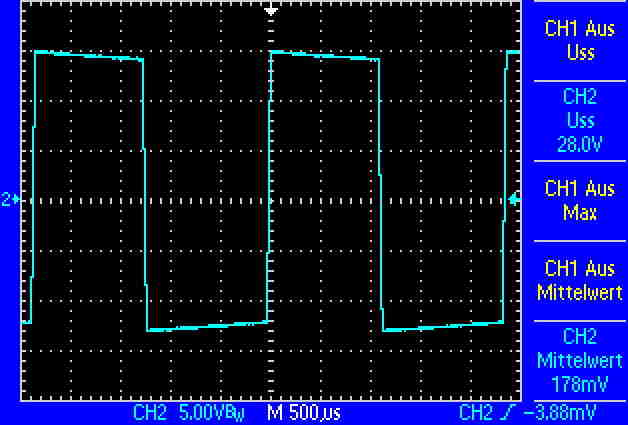
\includegraphics[width=.9\linewidth]{./img/ss-wavegen-squ}
		\caption{Square Wave Output Signal}
	\end{subfigure}
	\caption{Square and Triangle Wave Generator Waveforms}
	\label{ss:wavegen}
\end{figure}

\section{Programmable Differential Equation}


	%%!TEX root = ../10-Specific-Heat-Capacity.tex
\Appendix
\configureappendix

	%\TheBibliography
\bibliographystyle{babalpha}
\bibliography{../common/lit}

\end{document}
